\setcounter{chapter}{7}
\chapter{Simulation}
\label{cha:simulation_analysis}
% \minitoc
% 
% 
% 
This chapter contains focuses on the simulation of \ac{3D-PLI}.
For this the first part i about measuring every parameter from the experimental setup needed for the simulation.
The second part analysis the different bhaviers of the simulation parameters, such as the internal voxel size, and guids to a operating values.
The last parts takes a closer look at the results with the previous modeled two population fiber bundels.
% 
\section{Experimental Parameters}
% 
% 
% 
\subsection{optical resolution / convolution \texorpdfstring{\opticsigma{}}{}}
% 
Every optical microscope has imaging errors.
The most common are lens aberration, chromatic aberration, ...
All these errors lead to a reduced resolution.
The resolution for each experimental setup must therefore be determined.
For this purpose, the USAF test chart is very often used to characterize the resolution of an optical image setup.
It consists of multiple patterns, which have three slits with defined distances and widths.
The resolution can then be determined e.g. with the help of the Rayleigh criterion.
% 
\\
%
\begin{figure}[!t]
\centering

\subcaptionbox{microscopig image}[.45\textwidth]{
\begin{tikzpicture}[baseline]
    \node[anchor=south east,inner sep=0] at (0,0) {
    \scalebox{-1}[1]{\includegraphics[width=0.45\textwidth, trim = 919 1205 1029 743, clip, interpolate=false, ]{data/Taorad_USAF_AB4_LB85_5pct_5ms_a00_t000_1.png}}};
\begin{scope}[xscale=-1]
    % \draw[magenta,ultra thick,rounded corners] (0.25,0.5) rectangle (1.5,1.25);
    \draw[magenta,ultra thick,dashed,rounded corners] (0.25,0.5) rectangle (1.4,1.175);
    % \draw[yellow,ultra thick,rounded corners] (2,0.75) rectangle (3.15,1.5);
    \draw[yellow,ultra thick,dashed,rounded corners] (1.85,0.8) rectangle (2.9,1.4);
    % \draw[cyan,ultra thick,rounded corners] (3.0,2.3) rectangle (3.9,2.8);
    \draw[cyan,ultra thick,dashed,rounded corners] (2.75,2.1) rectangle (3.6,2.6);
    % \draw[green,ultra thick] (0,0) grid (5,5);
\end{scope}
\end{tikzpicture}
\hfill}
\subcaptionbox{line plots. \itodo{single line plots not good}}[.45\textwidth]{
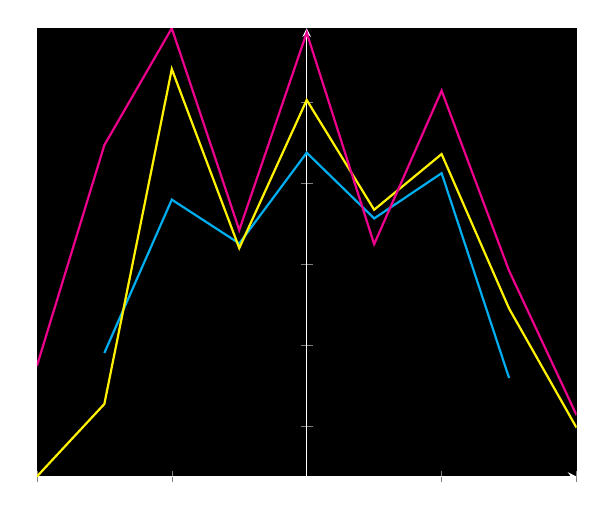
\begin{tikzpicture}[baseline]
\begin{axis}[%
axis x line = center,
axis y line = center,
xticklabels={,,},
yticklabels={,,},
scaled y ticks=false,
axis background/.style={fill=black},
axis line style={white},
]
\addplot [cyan, thick] coordinates {
(-3,	9530.667)
(-2,	19007.85)
(-1,	16297.67)
(0,	21909.00)
(1,	17846.71)
(2,	20642.69)
(3,	7984.000)
};
\addplot [yellow, thick] coordinates {
(-4,	1890.667)
(-3,	6374.111)
(-2,	27080.000)
(-1,	16011.000)
(0,	25166.666)
(1,	18383.334)
(2,	21824.000)
(3,	12277.556)
(4,	4910.222)
};
\addplot [magenta, thick] coordinates {
(-4,	8725.333)
(-3,	22378.074)
(-2,	29604.346)
(-1,	17126.518)
(0,	29328.791)
(1,	16255.111)
(2,	25744.297)
(3,	14614.123)
(4,	5688.889)
};
\end{axis}
\end{tikzpicture}
% \includegraphics[width=0.45\textwidth]{example-image}
}
\caption[USAF test chart measurement]{taorad pm. Line width: magenta: $\SI{2.19}{\micro\meter}$, yellow $\SI{1.95}{\micro\meter}$ and cyan $\SI{1.74}{\micro\meter}$. Resolution at about $\SI{1.95}{\micro\meter}$ yielding to an optical convolution of $\opticsigma = \SI{0.75}{\pixel}$.}
\label{fig:USAF}
\end{figure}
% 
\cref{fig:USAF} shows a section from a captured PM image. The highlighted areas show the key areas. A resolution of about $\SI{1.95}{\micro\meter}$ is estimated. Therefore the convolution to be applied has to be $\opticsigma = \SI{0.75}{\pixel}$ in the size of the resulting image pixel.
% 
% 
% 
\subsection{sensor gain}
%
\begin{figure}[!t]
\centering
\includegraphics[width=0.75\textwidth]{dev/gfx/2/PM_noise.png}
\caption[Noise analysis]{Noise analysis PM. $\opticgain_{\mathit{PM}} = \SI{0.1175}{}(?)$. \itodo{replot, also show microscope image}}
\label{fig:parameterModelSimGain}
\end{figure}
% 
As described in \cref{sec:ccdOptic} the optical oise has to be applied by a noise model.
In a former PhD Dissertation \cite{Wiese:887678} Hendrik Wiese measured the noise gain factor of the \ac{LAP} setup by measuring multiple times an image with a varieties of intensity values.
The same type of measurement and analysis is performed here on the \ac{PM} setup.
The results are shown in \cref{fig:parameterModelSimGain} and show a gain value of $\opticgain_{\mathit{PM}} = \SI{0.1175}{}(?)$ which is agreement to the hardware specifics \todo{check}.
% 
% 
% 
\subsection{Tissue}
% 
\begin{figure}[!tp]
\captionsetup[sub]{}%position=top
\subcaptionbox{\label{fig:human:transmittance}}[0.84\textwidth]{
% \fbox{
\begin{tikzpicture}[trim axis left, trim axis right]
\begin{axis}[%
width=0.84\textwidth,
% title = {$B_1^{equ}$ in $\mu T$},
xmin=0.5,xmax=1109.5,ymin=0.5,ymax=848.5,y dir=reverse,
% point meta min=0,point meta max=6370.19,
hide axis,
colormap/blackwhite,colorbar,
]
\addplot [forget plot] graphics [xmin=0.5,xmax=1109.5,ymin=0.5,ymax=848.5] {dev/gfx/data/Vervet1818a_60mu_70ms_s0549_x00-25_y00-33_thumbnail_Transmittance-1.png};
\draw[yellow, very thick, ->] (axis cs: 650,175) -- (axis cs: 586,265);
\draw[yellow, very thick]
(axis cs: 645.75,	295.575) --
(axis cs: 636.45,	272.375) --
(axis cs: 625.65,	275.975) --
(axis cs: 611.325,	275.175) --
(axis cs: 611.725,	300.275) -- cycle;
\draw[yellow, very thick]
(axis cs:551.9,290.75) --
(axis cs:561.05,269.6) --
(axis cs:548.45,265.7) --
(axis cs:537.35,257) --
(axis cs:523.4,278.3) -- cycle;
\end{axis}
\end{tikzpicture}
\label{fig:brain_trans}
}
\\[2em]
\subcaptionbox{}[0.84\textwidth]{
\begin{tikzpicture}[trim axis left, trim axis right]
\begin{axis}[%
width=0.84\textwidth,
% title = {$B_1^{equ}$ in $\mu T$},
xmin=0.5,xmax=1109.5,ymin=0.5,ymax=848.5,y dir=reverse,
% point meta min=0,point meta max=1.0,
hide axis,
colormap/blackwhite,colorbar,
]
\addplot [forget plot] graphics [xmin=0.5,xmax=1109.5,ymin=0.5,ymax=848.5] {dev/gfx/data/Vervet1818a_60mu_70ms_s0549_x00-25_y00-33_thumbnail_Retardation-1.png};
\draw[yellow, very thick, ->] (axis cs: 650,175) -- (axis cs: 586,265);
\draw[yellow, very thick]
(axis cs: 645.75,	295.575) --
(axis cs: 636.45,	272.375) --
(axis cs: 625.65,	275.975) --
(axis cs: 611.325,	275.175) --
(axis cs: 611.725,	300.275) -- cycle;
\draw[yellow, very thick]
(axis cs:551.9,290.75) --
(axis cs:561.05,269.6) --
(axis cs:548.45,265.7) --
(axis cs:537.35,257) --
(axis cs:523.4,278.3) -- cycle;
\end{axis}
\end{tikzpicture}
\label{fig:brain_ret}
}\hspace*{\fill}
 \caption[Vervet coronal section transmittance and retardation]{Vervet coronal section. a) Transmittane, b) Retardation. The absorption coefficient and birefingence strength can be estimated from flat fibers. The corpus calusum is in a coronal section suited for this. \itodo{histograms?}}
\label{fig:brain_ret_trans}
\end{figure}
% 
\begin{figure}[!tp]
\centering
\subcaptionbox{transmittance}[.95\textwidth]{
\includegraphics[width=0.95\textwidth]{dev/gfx/2/transmittance_PM_Vervet.pdf}} %\hfill
\subcaptionbox{retardation\label{fig:retValues}}[.95\textwidth]{
\includegraphics[width=0.95\textwidth]{dev/gfx/2/retardation_PM_Vervet.pdf}}
\caption{simulations for Vervet PM tissue for different absorption coef and birefringence values.}
\label{fig:parameterModelSim}
\end{figure}
% 
The physical proerty of the absorption coefficient  and the birefingence strenth \dn{} has to be estimated from the tissue to use fisable values inside the simulation.
This is easiest to be done from areas of flat fiber regions.
In a coronal section the corpus calosum is suited for this, since it is the main fiber connection between both brain hemispheres.
Problematic is in the transmittance that with this setup the scattering cant be distinguishable from the actual absorption.
However since this property is mathematically the same, a reduction of intensity along the tissue, it can be still used, but keeping in mind, that it is the overhaul "absorption" and not only the loos of energy inside the tissue.
Additionally one has to be keep in mind, that the scattering is not constant for all fiber configurations and orientations.
Therefore the measured value here is only valid for the same fiber configurations, as the region.
However it should be a good estimate of the order of absorption in the tissue, which will later shown in the simulation is already sufficient.
% \\
% 
% 
% 
\subsubsection{absorption}
% 
A relative transmittance of about $\SIrange{20}{30}{\percent}$ is inside the \ac{CC} \todo{show histogram}. 
The simulation parameter has to be set such as that for the models a similar transmittance value is reached.
To find this values the model of r=0.5 radii is used since it is closed to the real values.
% 
\ITODO{transmittance is twice as high as it should be !!! -> increase absorption coeeficient}

For r=0.5 and a Vfraction of 0.75 mu\_vervet = 30, mu\_human = 65, mu\_roden = 8
% 
% This yield to a absoprtion coefficient $\absorp_\textit{Vervet} = \SI{20}{\per\micro\meter}$. For the human and mouse a value of $\absorp_\textit{human} = \SI{50}{\per\micro\meter}$ and $\absorp_\textit{mouse} = \SI{10}{\per\micro\meter}$ is measured.
% 
% 
% 
\subsubsection{birefringence}
% 
Literature measured a birefringence of nerve fibers of around \dummy{}. 
Scince for this simulations the models are rigide and therefore are spatially farer away from each other, this means that the tissue density is lower than in reality.
Therefore to reach similar retardation values the birefringence value has to be increased.
For this purpuse retardation values with different birefringence values is simulated at a voxel size of \SI{0.125}{\micro\meter}.
The results shown in \cref{fig:retValues} show that to reach a retardation value similar to the experimental setup of around $\SI{0.8}{}$ a birefringence value of $\SI{-0.004}{}$ for a macroscopic and $\SI{0.008}{}$ for the microscopic model should be choosen.
Looking at the different model nerve fiber radii the variance of the retardation values increase strong.
This is to be expected since the simulated tissue section has a hight of $\SI{60}{\micro\meter}$.
Therefore for a radii of $\SI{10}{\micro\meter}$ the number of tissue voxels has to varry depending on where the fibers are positioned in the volume.
% 
\ITODO{effect of 0.75 radii?}
% 
% 
% 
\subsection{noise}
% 
\begin{figure}[!t]
\centering
% 
\begin{tikzpicture}[trim axis left, trim axis right]
\begin{loglogaxis}[%
xlabel={intensity},
ylabel={rel $\sigma$},
log ticks with fixed point,
ytick={0.01, 0.02, 0.03, 0.04},
]
% np.sqrt(x * 0.1175)/x
\addplot [%
BLUE, thick, smooth,
] coordinates {
(9.701e+01, 3.480e-02)
(2.048e+03, 7.574e-03)
};
\addplot+[%
RED, only marks, mark=*,
nodes near coords, node near coords style={anchor=south west},
point meta=explicit symbolic,
]
table[meta=label]{
x y label
115 0.0319 Human
574 0.01430 Vervet
1608 0.008548 Roden
};
\end{loglogaxis}
\end{tikzpicture}
% 
\caption[noise plot]{noise \dummy{}}
\label{fig:noiseplot}
\end{figure}
% 
Looking at the relative noise level for different species or absorptions, the relative noixe is between 1 and 4 percent for typical tissue sections.
For low intensity values however the digital discretication will be noticable.
This results can be transfert into retardation, meaning, that a retardation about the size of the realtive noise level cant be noticed.
% 
% 
% 
\subsection{voxel size \texorpdfstring{\voxels{}}{}}
% 
% % 
% In \cref{sec:dv_generator} the \voxelsize{} parameter $\voxels$ was introduced.
% This parameter has a major role in the accuracy of the results.
% It does not only account for the discretization accuracy of the 3d model, but also for the number of light rays.
% The impact is visualie shown in \cref{fig:vectorfield_disc_error}.
% It is cleare that 
% 
% TODO: anhang?
% \begin{figure}[p]
% \centering
% \includegraphics[width=\textwidth, page=4]{dev/gfx/2/voxel_size_plots_data_0.pdf}
% \caption[voxel size model without noise]{without noise \dummy{}}
% \label{fig:voxelsize}
% \end{figure}
% 
\begin{figure}[!tp]%p
\centering
\includegraphics[width=\textwidth, page=4]{dev/gfx/2/voxel_size_plots_data_1.pdf}
\caption[voxel size model with noise]{with noise \dummy{}}
\label{fig:voxelsizeNoise}
\end{figure}
% 
The voxel size \voxelsize{} is the main parameter for the simulation accuracy.
Smaller values mean more details, accurater optical axis, more light rays.
However this also mean an increas of memory of $O(n^3)$.
Therefore it is feasable to choose a voxel size as small as passible, with tolleratable results.
\\
% 
To investigate this effect a simulation is done with different kinds of voxel sizes from \SIrange{0.0125}{1.25}{\micro\meter}.
As \say{ground truth} the smallest voxel size \SI{0.0125}{\micro\meter} is used. 
However this voxel size is so small, this is done only for a single tissue section \itodo{which one?}.
\\
%
The results shown in \cref{fig:voxelsizeNoise} indicate that with noise a voxel size smaller than $\SI{0.125}{\micro\meter}$ does not increase the accuracy with respect to the noise model choosen here.
This however is only true for a pixel size of $\SI{1.25}{\micro\meter}$.
% 
% 
% 
\subsection{Fiber radii}
% 
\begin{figure}[!t]
\centering
\includegraphics[width=1\textwidth]{dev/gfx/sim_cube/radius_acc_compare_Vervet_PM_r.pdf}
\caption[sim acc]{sim\_acc, r0 = 0.5 \dummy{}. hypothese: abweichungen in GtSim bei kleinen radien dadurch, dass zwei richtungen nicht sichtbar sind? schaue dir die histogramme und odfs an.}
\label{fig:parameterModelSimGain}
\end{figure}
% 
% \itodo{zeige acc zwischen model r und p von simulationen an}
% 
\subsection{Fiber model}
% 
\itodo{warum eigentlich überhaupt p und r, warum nicht einfach nur r, und nur bei LAP r und p diskutieren? -> analysen (tilting) basieren auf p}
p ist bei grosen \say{fasern}, also FB sinnvoller, da hier auch steile fasern das signal verlieren. Bei radialen axen hingegen wäre das signal stark sichtbar.
% 
% 
% 
\newpage
% 
\section{Simulation}
% 
\begin{enumerate}
\item anfang
    \begin{enumerate}
    \item Welchen einflu\ss hat mu? theoretisch abhandelbar und unsicherheiten im vergleich.
    \item wie verh\"alt sich retardation als $f(\Psi, \Omega, ...)$
    \item ab welchem radius sind unterschiede bemerkbar? als erstes? welches kriterium?
    \end{enumerate}
% 
\item mitte
    \begin{enumerate}
    \item sekund\"are richtung sichtbar?
    \item Fom und modalit\"aten zeigen
    \item Histogramm der Modelle im vergleich zur Messung
    \item einfluss der inklination bei kreuzungen?
    \item Rofl abweichend bei starker Retardierung? Messungen ohne Rauschen ... auch Flache Messungen
    \item Rofl trel vergleich mit theo trel von gewebe dicke
    \end{enumerate}
% 
\item ende?
    \begin{enumerate}
    \item einfluss von model p auf tilt analyse?
    \item filled fibers?
    \item faser radien bei LAP(20 um)?
    \end{enumerate}
\end{enumerate}
% 
% 
% 
\subsection{Parameters}
% 
\begin{table}[!b]
\centering
\sisetup{open-bracket={\{}, close-bracket={\}}, list-final-separator={,},list-pair-separator={,}}%
\pgfplotstabletypeset[%
    thesisTableStyle,
    column type=l,
    columns/variable/.style={string type},
    columns/value/.style={string type},
    every head row/.style={before row=\toprule,after row=\midrule},
    every last row/.style={after row=\bottomrule},
    col sep=&,
    row sep=\\,
]
{variable & value\\
% 
simpli.voxel\_size & $\SI{0.125}{\micro\meter}$\\
simpli.pixel\_size & $\SI{1.25}{\micro\meter}$\\
simpli.voi & $[\SI{-30}{\micro\meter}, \SI{-30}{\micro\meter}, \SI{-30}{\micro\meter}], [\SI{30}{\micro\meter}, \SI{30}{\micro\meter}, \SI{30}{\micro\meter}]$\\
simpli.filter\_rotations & $\SIlist{0;20;40;60;80;100;120;160}{\degree}$\\
simpli.interpolate & \texttt{"Slerp"}\\
simpli.wavelength & $\SI{525}{\nano\meter}$\\
simpli.optical\_sigma & $\SI{0.75}{\pixel}$\\
tilt & $\SI{3.9}{\degree}$\\
simpli.light\_intensity & $\SI{8000}{}$\\
gain & $\SI{0.1175}{}$\\
% simpli.noise\_model & \texttt{lambda x:np.round(np.random.normal(x,np.sqrt(gain * x))).astype(np.uint16)}\\
simpli.noise\_model & \texttt{lambda x:np.round(np.random.normal(}\\
 & \ \ \ \ \ \texttt{x,np.sqrt(gain * x))).astype(np.uint16)}\\
fiber absorption & ('Roden', 10), ('Vervet', 20), ('Human', 50)\\
fiber model & 'p' and 'r'\\
fiber birefringence & -0.004 and 0.008\\
fiber radii & 0.75 and  1\\
}
\caption{simpli parameters. \ITODO{to low because of tissue spacing}}
\label{tab:simParameters}
\end{table}
% 
% 
% 
\subsection{expected results}
% 
% 
% 
\subsection{Results}
% 
\itodo{other results?}
\begin{itemize}
\item noise(omega, gamma, ...)
\item second orientation visible?
\item absolute birefringence, transmittance, absorption as a f(omega)
\item trel? abnahme der doppelbrechnung in flachen faser, bzw gegenüber f0?
\end{itemize}
% 
% 
% 
\subsection{Retardation comparison}
% 
\begin{figure}[!t]
\centering
\inputtikz{dev/gfx/sim_cube/data_rofl}
% \includegraphics[width=0.75\textwidth]{example-image} 
\caption[data vs rofl]{data vs rofl}
\label{fig:sim_05_PM_Vervet_r_r}
\end{figure}
\itodo{show sinus plot of single pixel}
% 
\begin{figure}[!tp]
\centering
\includegraphics[width=\textwidth]{dev/gfx/sim_cube/simulation_retardation_PM_Vervet_r.pdf}
% 
\begin{tikzpicture}
 \begin{axis}[
 scale only axis, width=0pt, height=0pt, hide axis,
 tick label style={/pgf/number format/.cd, fixed},
 colorbar,colormap/viridis high res,
 point meta min=0,
 point meta max=1,
  colorbar horizontal,
  colorbar style={width=0.75\textwidth},
  ]%
  {};
 \end{axis}
\end{tikzpicture}
% 
\caption[simulation results retardation]{0.5, PM, Vervet, r, retardation  \dummy{}}
\label{fig:sim_retardation_05_PM_Vervet_r}
\end{figure} 
% 
% 
% 
\subsection{Orientation comparison}
% 
\begin{figure}[!tp]
\centering
\includegraphics[width=\textwidth, trim = 115 50 115 0, clip]{dev/gfx/sim_cube/tissue_overlay_PM_Vervet_r_0.60_60.00_10.00_30.00_0.00_.pdf} 
\caption[sim]{\dummy{}}
\label{fig:sim_fyjsrg}
\end{figure}
% 
% 
% 
\begin{figure}[!t]
\begin{tikzpicture}[trim axis left, baseline]
\begin{axis}[%
    axis equal,
    axis lines = center,
    axis line style={opacity=0.0},
    ticks=none,
    view/h=145,
    scale uniformly strategy=units only,
    clip=false, % hide axis,
    width=10cm,
    height=10cm,
    xmin=-1,xmax=1,
    ymin=-1,ymax=1,
    zmin=-1,zmax=1,
    point meta min=0, point meta max=1,
    colormap/viridis,
]
\addplot3[%
    surf,
    shader=interp,
    z buffer=sort,
    mesh/color input=explicit,
    ]
 table[x=x,y=y,z=z,
        meta=rgb,
        ] {dev/gfx/sim_cube/cube_2pop_psi_0.60_omega_60.00_r_10.00_v0_120_.solved_vs_0.1250_inc_30.00_rot_0.00_PM_Vervet_r.gt.dat};
\end{axis}
\end{tikzpicture}
\begin{tikzpicture}[trim axis left, baseline]
\begin{axis}[%
    axis equal,
    axis lines = center,
    axis line style={opacity=0.0},
    ticks=none,
    view/h=145,
    scale uniformly strategy=units only,
    clip=false, % hide axis,
    width=10cm,
    height=10cm,
    xmin=-1,xmax=1,
    ymin=-1,ymax=1,
    zmin=-1,zmax=1,
    point meta min=0, point meta max=1,
    colormap/viridis,
]
\addplot3[%
    surf,
    shader=interp,
    z buffer=sort,
    mesh/color input=explicit,
    ]
 table[x=x,y=y,z=z,
        meta=rgb,
        ] {dev/gfx/sim_cube/cube_2pop_psi_0.60_omega_60.00_r_10.00_v0_120_.solved_vs_0.1250_inc_30.00_rot_0.00_PM_Vervet_r.rofl.dat};
\end{axis}
\end{tikzpicture}
% 
\caption[odf]{\dummy{}}
\label{fig:sim_fyjsrg}
\end{figure}
% 
% 
% 
% 
\begin{figure}[!tp]
\centering
\includegraphics[width=\textwidth]{dev/gfx/sim_cube/simulation_analysis_hist_0.5_setup_PM_s_Vervet_m_r_acc.pdf}
% 
\begin{tikzpicture}
 \begin{axis}[
 scale only axis, width=0pt, height=0pt, hide axis,
 tick label style={/pgf/number format/.cd, fixed},
 colorbar,colormap/viridis high res,
 point meta min=0,
 point meta max=1,
  colorbar horizontal,
  colorbar style={width=0.75\textwidth,},
  ]%
  {};
 \end{axis}
\end{tikzpicture}
% 
\caption[simulation results mean diff]{0.5, PM, Vervet, r, acc-distance: interpolated grid,  \dummy{}. \say{SPOTS only a interpolation artefact!}}
\label{fig:sim_05_PM_Vervet_r_r}
\end{figure}
% 
\itodo{unterschied rofl ungenauigkeit mit einer faser zu 2 fasern}

% 
% \itodo{abosulte accurracy}
% 
% 
% 
\subsubsection{different species / transmittance}
% 
% 
% 
\subsubsection{parallel model}
% 
% 
% 
\subsubsection{LAP}